% Information Sciences
\documentclass[11pt]{article}

\usepackage[margin=1in]{geometry}
\usepackage{amsmath,amssymb,amsthm}
\usepackage{booktabs}
\usepackage{graphicx}
\usepackage{algorithm}
\usepackage{algpseudocode}
\usepackage[numbers,sort&compress]{natbib}
\usepackage[colorlinks=true,citecolor=blue,linkcolor=blue,urlcolor=blue]{hyperref}
\emergencystretch=2em

\newtheorem{theorem}{Theorem}
\newtheorem{lemma}{Lemma}
\newtheorem{proposition}{Proposition}
\newtheorem{assumption}{Assumption}

% --- headline numbers from results/method_means.csv + summary.csv (5 seeds) ---
\newcommand{\CodaMean}{26.8}
\newcommand{\CodaPmiss}{0.05}
\newcommand{\CodaUpload}{0.015}
\newcommand{\CodaEnergyMJ}{13}
\newcommand{\CodaExit}{97}
\newcommand{\CodaSelErr}{6.7}
\newcommand{\CodaAcc}{92.6}
\newcommand{\CloudMean}{109}
\newcommand{\CloudPmiss}{52}
\newcommand{\CloudUpload}{2}
\newcommand{\LocalEnergyMJ}{31}
\newcommand{\ConfExitMean}{28}
\newcommand{\ConfExitMiss}{1.5}
\newcommand{\CongCloudMiss}{83}
\newcommand{\CongConfMiss}{2.5}
\newcommand{\CongCodaMiss}{0.0}
\newcommand{\LocalFullMs}{61}
\newcommand{\EdgeGflops}{5}

\title{CODA-SC: Calibrated Selective Edge-Cloud Inference Under Internet Deadlines}
\author{Anonymous Authors}
\date{}

\begin{document}
\maketitle

\begin{abstract}
Edge-cloud inference must decide whether to answer locally, offload remotely, or
use a local fallback under predictive uncertainty and variable Internet latency.
Existing split-computing methods mainly optimize profiled systems costs, whereas
early-exit methods often rely on uncalibrated confidence thresholds. We propose
CODA-SC, a calibrated selective edge-cloud inference framework for multi-exit
CNNs. CODA-SC accepts a local exit only when the conformal prediction set is a
singleton; otherwise, a primal-dual controller selects a remote split or local
fallback using latency, upload, energy, and deadline feedback. We establish
finite-sample coverage and selective-error bounds for the exits and analyze an
idealized binary-slack controller with $O(\sqrt{T})$ regret and constraint
violation under bounded feedback. Using measured CNN FLOPs and activation
payloads with simulated Internet-like traces across four vision workloads, four
network profiles, five seeds, and twelve policies, CODA-SC-Cov reduces mean
latency from \CloudMean~ms to \CodaMean~ms and deadline misses from
\CloudPmiss\% to \CodaPmiss\%, with \CodaUpload~KB upload and about a two-point
accuracy reduction. CODA-SC-Risk trades latency for lower selective error and
higher accuracy. A learned-bottleneck split study further tests compressed
intermediate actions while retaining the device-model and trace-simulation
scope. These results support calibrated selective control, not hardware
deployment validation.
\end{abstract}

\noindent\textbf{Keywords:} split computing; conformal prediction; edge
intelligence; online optimization; reliable machine learning; intelligent
systems

\section*{Highlights}
\begin{itemize}
    \item Conformal exits calibrate selective edge-cloud inference.
    \item A primal-dual controller handles deadline-critical residual samples.
    \item CNN FLOPs and activation payloads are measured, not hand-set.
    \item Learned bottlenecks test compressed intermediate split actions.
    \item Reproducible code regenerates tables, figures, and diagnostics.
\end{itemize}

\section{Introduction}

Edge-cloud inference systems must decide where a neural-network request should
be executed. Cloud-only inference preserves the accuracy of the full model, but
each request incurs uplink transmission, round-trip delay, queueing, and loss.
Local-only inference avoids network uncertainty, but it consumes device compute
and energy. Split computing introduces intermediate actions: execute a prefix on
the device, transmit the activation, and complete the suffix remotely. Multi-exit
networks add sample-adaptive local decisions, allowing easy examples to terminate
before either the full local model or the network is used.

The standard formulation treats these decisions separately. Split-computing
systems such as Neurosurgeon \citep{kang2017neurosurgeon}, Edgent
\citep{li2019edgent}, and Auto-Split \citep{banitalebi2021autosplit} profile
layer compute, payloads, and bandwidth to select a partition. Early-exit systems
classify samples at intermediate heads when a confidence score exceeds a
threshold \citep{teerapittayanon2017ddnn, teerapittayanon2016branchynet,
matsubara2022split}. Online partitioning methods further adapt to unknown delay
\citep{saxena2025aodpart}. These lines of work address important parts of the
pipeline, but they leave a coupled reliability question unresolved: when an
intermediate classifier is uncertain and the network is also uncertain, the
system must decide whether to exit, offload, or pay for a local full-model
fallback.

This coupling matters because the two uncertainties fail in different ways. A
confidence threshold can have favorable empirical accuracy on calibration data
without finite-sample coverage on future samples. A split policy can minimize
expected latency while still violating a hard deadline during queueing spikes.
The resulting deployment failure is not simply excessive mean latency; it is a
request-level decision error in which the system either trusts an unreliable
early prediction or sends an uncertain sample into a network path that is already
unlikely to meet the deadline.

We study this decision as a selective-prediction and constrained online-control
problem. CODA-SC wraps each intermediate exit in split conformal prediction
\citep{angelopoulos2021gentle}, so a local prediction is accepted only through a
calibrated prediction-set rule. Samples not accepted by the exits are assigned by
a primal-dual controller over remote split points and a local full-model
fallback. The controller estimates latency from measured local compute,
activation payload, bandwidth, RTT, queueing, and cloud suffix compute, and uses a
virtual deadline queue to penalize actions that are likely to exceed the deadline
budget. Thus, statistical uncertainty determines whether an early exit is
eligible, while online network feedback determines how to serve the remaining
requests.

The empirical evaluation is designed to avoid a common ambiguity in
split-computing studies: conclusions driven by hand-set payload and compute
constants. We train multi-exit convolutional networks on four vision workloads.
Activation payloads are exact int8 tensor sizes, and compute latency and energy
are derived from measured per-stage FLOPs under a documented edge/cloud device
model. Network variability is evaluated with simulated Internet-like traces that
include bandwidth, RTT, queueing, and loss; therefore the absolute network
latencies should be interpreted as trace-simulation results, while the model-side
costs are measured from the trained networks.

The resulting contribution is positioned as an intelligent-systems decision
method rather than a network protocol. CODA-SC combines uncertainty
quantification, online optimization, and resource-aware deep inference:
conformal prediction specifies when an intermediate representation is informative
enough to leave the device as a label, while the controller determines when the
information should be transmitted, retained locally, or completed by the
full-model fallback. The contribution therefore lies at the interface between
machine learning, information processing, and adaptive computational-resource
allocation, rather than in network protocol design alone.

This paper makes the following contributions.

\begin{itemize}
    \item We formulate deadline-constrained edge-cloud inference as a joint
    selective-prediction and online-control problem over calibrated early exits,
    remote split points, and a local full-model fallback.
    \item We introduce CODA-SC, which combines conformal and conformal-risk-control
    exit rules with a deadline- and energy-aware primal-dual controller.
    \item We establish finite-sample coverage and selective-error bounds for the
    exit rules and analyze an idealized binary-slack controller with
    $O(\sqrt{T})$ regret and deadline-violation bounds under bounded feedback and
    latency-estimation error.
    \item We evaluate the method in a model-measured, trace-simulated benchmark
    with measured CNN FLOPs and activation payloads across four vision workloads,
    four network profiles, five seeds, and twelve policies, and add a learned
    bottleneck study that exposes the accuracy-latency trade-off of compressed
    split actions without claiming hardware deployment evidence.
\end{itemize}

\section{Related Work}

\paragraph{Split and collaborative inference.}
DDNNs \citep{teerapittayanon2017ddnn} introduced a hierarchy in which end,
edge, and cloud components can all participate in inference. Neurosurgeon
\citep{kang2017neurosurgeon} built layer-level latency and energy models to
choose mobile-cloud partitions. Edgent \citep{li2019edgent} jointly considered
partitioning and right-sizing through early exits under changing bandwidth.
Auto-Split \citep{banitalebi2021autosplit} turned collaborative edge-cloud AI
into an automated deployment pipeline. Recent systems extend the design space to
platform-agnostic partitioning \citep{partnner2024}, memory-limited devices
\citep{li2024flexnn}, near-edge accelerators \citep{liu2024near}, and dynamic
just-in-time edge execution \citep{inferedge2025}. These systems establish that
partition choice must depend on compute and network state, but their decisions
are typically made from profiled latency, bandwidth, or queueing models rather
than calibrated prediction sets. When intermediate activations are larger than
the input, learned bottlenecks such as BottleNet++ \citep{shao2020bottlenet}
compress the transmitted representation. CODA-SC is compatible with such
compression: the main benchmark isolates control and calibration, and the
additional bottleneck study tests whether compressed intermediate actions become
active under the same controller.

\paragraph{Early exit and adaptive computation.}
Early-exit models attach intermediate classifiers to reduce average inference
cost for easy samples \citep{teerapittayanon2016branchynet}. Surveys identify the
accuracy-latency trade-off and the need to jointly tune exits and split points
\citep{matsubara2022split}. Combining DNN partitioning with early exit adds
flexibility but is often driven by performance models or confidence heuristics
\citep{veith2022combining}. Calibration work argues that confidence alone is not
the whole early-exit problem, because the decision should account for whether
continuing computation is worth its cost \citep{kubaty2025rethinking}. CODA-SC
differs by making the exit decision a conformal prediction-set decision. The
advantage is not a claim of lower error than every confidence threshold; rather,
it is an explicit finite-sample reliability statement and a
controlled abstention mechanism that can be composed with online offloading.

\paragraph{Network robustness and online offloading.}
Packet-loss-tolerant split inference trains models to survive missing activation
packets without retransmission \citep{itahara2021packet}. AODPart
\citep{saxena2025aodpart} models partitioning with early exits and unknown
communication/processing delay as online delay-constrained accuracy
maximization. In-network split inference explores programmable network nodes and
Named Data Networking under lossy edge connectivity \citep{ndn2025split}. CODA-SC
targets a different failure mode: it couples a statistically calibrated exit rule
with a deadline-aware controller and local fallback. This is complementary to
compression, packet-loss robustness, and in-network placement. We compare
directly against a reimplementation of the AODPart online-partitioning idea to
separate the effect of online delay control from the effect of conformal
selective prediction. This comparison is important because AODPart-style control
can match CODA-SC on latency and deadline misses in some regimes; CODA-SC's
distinct contribution is the calibrated exit interface, the CRC selective-error
variant, and explicit upload minimization through $\gamma b_k$, not an
unconditional improvement in every systems metric.

\paragraph{Foundation-model split inference.}
Large foundation models create new split-computing regimes, including dynamic
edge orchestration \citep{koch2025adaptive} and WAN LLM split inference with
speculative decoding \citep{cunningham2026privacy}. These works show that
wide-area networking is a first-order bottleneck. CODA-SC targets feed-forward
classification in this manuscript; extending the method to autoregressive
decoding requires new actions for token-level scheduling, KV-cache placement, and
speculative execution.

\paragraph{Conformal prediction and risk control.}
Conformal prediction converts black-box model scores into prediction sets with
finite-sample, distribution-free coverage under exchangeability
\citep{angelopoulos2021gentle}. Conformal risk control generalizes this idea to
expected monotone losses \citep{angelopoulos2024crc}. CODA-SC uses conformal
sets to decide when an intermediate prediction may safely leave the device as a
point prediction, and uses conformal risk control to target selective error
directly. The coverage statement is marginal and depends on exchangeability; the
experiments therefore report calibration diagnostics rather than treating the
theory as evidence of robustness under arbitrary distribution shift.

\section{Problem Definition}

We consider a request stream $(X_t,Y_t)$ and a time-varying network process
observed online. The exchangeability assumption used for conformal calibration
applies to the labeled examples, not to the network process. A neural model has
$m$ local exits, $K$ offloading split actions, and a local full-model action.
Exit $e$ produces class probabilities $p_e(y\mid x)$ after local prefix compute
of $a_e$ FLOPs. Split action $k$ executes a local prefix of $u_k$ FLOPs, uploads
an activation of size $b_k$, and executes a cloud suffix of $v_k$ FLOPs.

Latency and energy are derived from measured model FLOPs and activation payloads
under a specified device model. Let the edge and cloud sustain
$\Phi_{\mathrm{e}}$ and $\Phi_{\mathrm{c}}$ FLOP/s. For split $k$, the realized
latency is
\begin{equation}
    L_t(k) = \frac{u_k}{\Phi_{\mathrm{e}}} + \frac{v_k}{\Phi_{\mathrm{c}}}
    + R_t + Q_t + \frac{8 b_k}{B_t}\cdot\frac{1}{1-\ell_t},
    \label{eq:latency}
\end{equation}
where $B_t$ is uplink bandwidth in Mbps, $R_t$ is round-trip time, $Q_t$ is
queueing delay, $\ell_t$ is loss probability, and $b_k$ is measured in KB. A local
exit at $e$ has latency $a_e/\Phi_{\mathrm{e}}$ and zero upload; the local
full-model fallback has latency $F/\Phi_{\mathrm{e}}$ where $F$ is the full-model
FLOPs. Edge energy of an action is $E(k)=u_k\,\varepsilon_{\mathrm{e}} +
b_k\,\varepsilon_{\mathrm{up}}$, with $\varepsilon_{\mathrm{e}}$ the edge
energy per FLOP and $\varepsilon_{\mathrm{up}}$ the upload energy per KB.

The online objective is to minimize a long-run cost combining latency, edge
energy, and upload while satisfying a deadline budget. Let
$M_t = \mathbb{1}\{L_t > D\}$ be the deadline miss. A target miss budget $\rho$
requires
\begin{equation}
    \frac{1}{T}\sum_{t=1}^{T} \mathbb{E}[M_t] \leq \rho.
\end{equation}
For local exits, prediction reliability is controlled separately: the system
emits a local point prediction only when the conformal set satisfies the exit
rule. This separation is essential. A split action controls latency and energy
but does not change the classifier's uncertainty; an exit action controls
communication and compute but must be statistically justified.

\section{CODA-SC}

\subsection{Conformal Exit Calibration}

For each exit $e$, define the nonconformity score
\begin{equation}
    S_e(x,y) = 1 - p_e(y\mid x).
\end{equation}
Given a calibration set $\mathcal{C}=\{(x_i,y_i)\}_{i=1}^{n}$ and target
miscoverage $\alpha$, CODA-SC computes
\begin{equation}
    q_e = S_{e,(\lceil (n+1)(1-\alpha)\rceil)},
\end{equation}
the conformal quantile of calibration scores at exit $e$. At inference, exit
$e$ returns the prediction set
\begin{equation}
    \Gamma_e(x) = \{y \in \mathcal{Y}: 1 - p_e(y\mid x) \leq q_e\}.
\end{equation}
CODA-SC answers locally at the first $e$ for which $|\Gamma_e(x)|=1$; otherwise
it invokes the online controller. This rule converts early exiting from an
uncalibrated confidence comparison into a prediction-set decision. As an
alternative that targets selective error directly, CODA-SC also supports a
conformal-risk-control threshold $q_e^{\star}$ chosen so that the calibration
singleton error, inflated by a finite-sample slack, is at most a target $\delta$
(Proposition~\ref{prop:crc}).

\subsection{Coupled Deadline-Aware Control}

CODA-SC maintains exponential moving estimates $\widehat{B}_t$,
$\widehat{R}_t$, and $\widehat{Q}_t$ from recent offloaded requests. The
estimated latency of split $k$ is
$\widehat{L}_t(k) = u_k/\Phi_{\mathrm{e}} + v_k/\Phi_{\mathrm{c}} + \widehat{R}_t
+ \widehat{Q}_t + 8b_k/\widehat{B}_t$, and the local fallback has fixed latency
$F/\Phi_{\mathrm{e}}$. CODA-SC keeps a dual variable $\lambda_t$ for deadline
pressure and, over the action set $\mathcal{A}$ of split points \emph{and} the
local fallback, selects
\begin{equation}
    k_t = \arg\min_{k\in\mathcal{A}} \widehat{L}_t(k)
          + \lambda_t [\widehat{L}_t(k)-D]_+
          + \beta E(k) + \gamma b_k.
    \label{eq:controller}
\end{equation}
After observing realized latency $L_t(k_t)$, it updates
\begin{equation}
    \lambda_{t+1} = [\lambda_t + \eta(\mathbb{1}\{L_t(k_t)>D\}-\rho)]_+.
    \label{eq:dual}
\end{equation}
The coupling to the exits has two functions. First, including the local fallback
in $\mathcal{A}$ lets the same dual $\lambda_t$ that tracks the deadline budget
decide between offloading, which is energy-cheap but network-dependent, and local
execution, which is deadline-safe but energy-expensive. Second, because local
exits are admitted only through singleton conformal sets, the controller acts
only on samples for which the intermediate classifiers did not provide a
calibrated point prediction. The virtual queue increases the penalty on risky
offloads after deadline misses and reduces it when recent requests satisfy the
budget.

\begin{algorithm}[t]
\caption{CODA-SC Inference}
\label{alg:coda}
\begin{algorithmic}[1]
\Require exits $e=1,\ldots,m$, actions $\mathcal{A}$ (splits + local fallback),
conformal quantiles $\{q_e\}$, deadline $D$, miss budget $\rho$
\State initialize network estimates $\widehat{B},\widehat{R},\widehat{Q}$ and dual $\lambda\gets0$
\For{request $x_t$}
    \For{exit $e=1,\ldots,m$}
        \State compute $p_e(\cdot\mid x_t)$ and $\Gamma_e(x_t)=\{y:1-p_e(y\mid x_t)\le q_e\}$
        \If{$|\Gamma_e(x_t)|=1$}
            \State \Return $\arg\max_y p_e(y\mid x_t)$ locally
        \EndIf
    \EndFor
    \For{action $k\in\mathcal{A}$}
        \State estimate $\widehat{L}_t(k)$ and score $J_t(k)=\widehat{L}_t(k)+\lambda[\widehat{L}_t(k)-D]_+ + \beta E(k)+\gamma b_k$
    \EndFor
    \State choose $k_t=\arg\min_k J_t(k)$; offload at split $k_t$ or run the local fallback
    \State observe latency $L_t(k_t)$; update $\widehat{B},\widehat{R},\widehat{Q}$
    \State $\lambda\gets[\lambda+\eta(\mathbb{1}\{L_t(k_t)>D\}-\rho)]_+$
\EndFor
\end{algorithmic}
\end{algorithm}

\section{Theoretical Analysis}

\begin{assumption}[Exchangeable calibration]
For each exit $e$, the calibration examples and the future test example are
exchangeable with respect to the nonconformity score $S_e(X,Y)$.
\end{assumption}

\begin{theorem}[Conformal exit coverage]
\label{thm:cov}
For any exit $e$ calibrated as above, $\mathbb{P}\{Y \in \Gamma_e(X)\} \geq 1-\alpha$.
\end{theorem}
\begin{proof}
This is the standard split-conformal classification result: under
exchangeability the rank of the test score among the $n$ calibration scores is
uniform up to ties, so the $\lceil(n+1)(1-\alpha)\rceil$ calibration quantile
yields marginal coverage at least $1-\alpha$. We state it to fix the exit
interface; the contribution is its use for selective offloading, not the bound.
\end{proof}

\begin{proposition}[Single-exit false singleton bound]
\label{prop:single}
Let $A_e=\{|\Gamma_e(X)|=1\}$ and let $\hat{Y}_e$ be the singleton label. Then
$\mathbb{P}(A_e \cap \{\hat{Y}_e \neq Y\}) \leq \alpha$, and if
$\mathbb{P}(A_e)>0$, $\mathbb{P}(\hat{Y}_e\neq Y \mid A_e) \leq \alpha/\mathbb{P}(A_e)$.
\end{proposition}
\begin{proof}
When $\Gamma_e(X)$ is a singleton and the label is wrong, the true label is not in
$\Gamma_e(X)$, so $A_e \cap \{\hat{Y}_e \neq Y\}\subseteq \{Y\notin\Gamma_e(X)\}$,
whose probability is at most $\alpha$ by Theorem~\ref{thm:cov}. Dividing by
$\mathbb{P}(A_e)$ gives the conditional statement.
\end{proof}

\begin{proposition}[Sequential-exit false singleton bound]
\label{prop:seq}
If exit $e$ is calibrated at level $\alpha_e$ and CODA-SC returns the first
singleton among $m$ exits, then the probability of returning any wrong singleton
is at most $\sum_{e=1}^{m}\alpha_e$.
\end{proposition}
\begin{proof}
A wrong accepted singleton at exit $e$ implies $Y\notin\Gamma_e(X)$; the event of
any wrong accepted singleton is a subset of $\cup_{e=1}^{m}\{Y\notin\Gamma_e(X)\}$,
and a union bound with Theorem~\ref{thm:cov} gives the result.
\end{proof}

\begin{proposition}[Conformal-risk-control selective error]
\label{prop:crc}
Fix exit $e$, target $\delta$, confidence level $\zeta$, and a finite threshold
grid $\mathcal{Q}$. Let $\widehat{r}(q)$ be the empirical singleton selective
error on $n_e(q)$ calibration singletons at threshold $q$. Choose the largest
$q^{\star}\in\mathcal{Q}$ satisfying
\begin{equation}
    \widehat{r}(q^{\star})+
    \sqrt{\frac{\log(|\mathcal{Q}|/\zeta)}{2n_e(q^{\star})}}\le\delta .
\end{equation}
Then, with probability at least $1-\zeta$, the population singleton selective
error at $q^{\star}$ is at most $\delta$.
\end{proposition}
\begin{proof}
For a fixed threshold, singleton correctness indicators are i.i.d.\ Bernoulli, so
Hoeffding's inequality gives
$\mathbb{P}(r(q)>\widehat{r}(q)+\sqrt{\log(|\mathcal{Q}|/\zeta)/(2n_e(q))})\le
\zeta/|\mathcal{Q}|$. A union bound over all $q\in\mathcal{Q}$ controls the
data-dependent choice of $q^{\star}$, and the defining inequality for
$q^{\star}$ gives the claim.
\end{proof}

\begin{assumption}[Bounded feedback and feasibility]
\label{ass:bounded}
The action set $\mathcal{A}$ is finite. For every action $k$ and time $t$, the
instantaneous cost $c_t(k)\in[0,C]$ and the constraint slack
$g_t(k)=\mathbb{1}\{L_t(k)>D\}-\rho\in[-1,1]$. There exists an admissible
comparison policy $\pi^{\star}$, using the same information as the controller, and slack
$\epsilon>0$ with
$\mathbb{E}[g_t(\pi^{\star})\mid\mathcal{H}_{t-1}]\le-\epsilon$ for every $t$
(conditional Slater feasibility). Latency estimates satisfy
$|\widehat{L}_t(k)-L_t(k)|\le\xi_t$; write
$\bar\xi=\frac1T\sum_t\mathbb{E}[(1+\lambda_t)\xi_t]$ for the weighted average
latency-estimation error incurred by the controller.
\end{assumption}

For the analysis, define the realized and estimated costs as
$c_t(k)=L_t(k)+\beta E(k)+\gamma b_k$ and
$\widehat{c}_t(k)=\widehat{L}_t(k)+\beta E(k)+\gamma b_k$, and define the binary
deadline slacks as
$g_t(k)=\mathbb{1}\{L_t(k)>D\}-\rho$ and
$\widehat{g}_t(k)=\mathbb{1}\{\widehat{L}_t(k)>D\}-\rho$.

\paragraph{Scope of analysis.}
The theorem below analyzes the binary-slack primal-dual abstraction of CODA-SC,
where deadline pressure enters through $\widehat{g}_t(k)$. The implementation
uses the hinge term $[\widehat{L}_t(k)-D]_+$ in Eq.~\eqref{eq:controller} as a
graded surrogate so that actions far beyond the deadline are penalized more
heavily than near-miss actions. The result therefore supports the constrained
online-control mechanism under bounded feedback and latency-estimation error,
while threshold flips for actions within $\xi_t$ of $D$ are absorbed into the
$T\bar\xi$ term.

\begin{theorem}[Idealized online deadline control]
\label{thm:online}
Under Assumption~\ref{ass:bounded}, the controller of
Eqs.~\eqref{eq:controller}--\eqref{eq:dual}, with the binary estimated slack
$\widehat{g}_t$ in the Lagrangian and step size $\eta=\Theta(T^{-1/2})$,
satisfies, in expectation,
\begin{equation}
    \mathbb{E}\!\left[\sum_{t=1}^{T}\!\big(c_t(k_t)-c_t(\pi^{\star})\big)\right]\le O(\sqrt{T})+T\bar\xi,
    \qquad
    \mathbb{E}\!\left[\sum_{t=1}^{T}\!\big(\mathbb{1}\{L_t(k_t)>D\}-\rho\big)\right]\le O(\sqrt{T})+T\bar\xi.
\end{equation}
\end{theorem}
\begin{proof}
Let $\Phi(\lambda)=\tfrac12\lambda^2$. Squaring Eq.~\eqref{eq:dual} and using
$[x]_+^2\le x^2$ and $|g_t|\le1$ gives the drift
$\Phi(\lambda_{t+1})-\Phi(\lambda_t)\le \eta\,\lambda_t g_t(k_t)+\tfrac12\eta^2$.
Because $k_t$ minimizes the estimated Lagrangian $\widehat c_t(k)+\lambda_t\widehat g_t(k)$
and the estimates deviate from the truth by at most $\xi_t$, for any fixed policy
$\pi$ we have
$c_t(k_t)+\lambda_t g_t(k_t)\le c_t(\pi)+\lambda_t g_t(\pi)+2(1+\lambda_t)\xi_t$.
Adding $\eta$ times this bound to the drift and telescoping over $t$ with
$\lambda_1=0$, $\Phi\ge0$ yields
\[
\sum_{t}\big(c_t(k_t)-c_t(\pi)\big)\le
\sum_t \lambda_t g_t(\pi) + \tfrac12\eta T + 2\sum_t(1+\lambda_t)\xi_t .
\]
Taking conditional expectations with $\pi=\pi^{\star}$ and using conditional
Slater feasibility gives
$\mathbb{E}[\lambda_t g_t(\pi^{\star})]\le-\epsilon\mathbb{E}[\lambda_t]$.
This term is non-positive and, by the standard finite-action
drift-plus-penalty stability lemma under Slater feasibility, the expected dual
queue remains stable rather than requiring pointwise feasibility of
$\pi^{\star}$ \citep{yu2017online}. Therefore, with
$\eta=\Theta(T^{-1/2})$, the expected cost regret is
$O(\sqrt T)+2\sum_t\mathbb{E}[(1+\lambda_t)\xi_t]=O(\sqrt T)+T\bar\xi$.
For the constraint, $[x]_+\ge x$ gives $\lambda_{t+1}\ge\lambda_t+\eta g_t(k_t)$,
so summing and taking expectations yields
$\mathbb{E}[\sum_t g_t(k_t)]\le\mathbb{E}[\lambda_{T+1}]/\eta$. The same Slater
stability argument bounds the expected terminal queue, giving
$O(\sqrt T)$ constraint violation, and the estimated-latency decisions add
$T\bar\xi$. This is the standard constrained primal-dual/drift-plus-penalty
result under Slater feasibility \citep{yu2017online}, specialized to a finite
action set; the non-standard term is the additive estimation-error penalty from
acting on $\widehat{L}_t$ rather than $L_t$.
\end{proof}

\section{Experiments}

\subsection{Experimental Setup}

We train a multi-exit convolutional network on four vision workloads that span a
difficulty range: MNIST, Fashion-MNIST, CIFAR-10, and SVHN. The backbone is a
compact VGG-style network with three convolutional blocks (channel widths
$64/128/256$) and three early-exit heads after blocks 1--3, trained with a
weighted multi-exit cross-entropy loss. Offloading actions are raw-input/cloud,
split after block 1, split after block 2, split after block 3, and local
full-model fallback. A held-out calibration split, drawn from the same data
generation process as the test stream, is used for conformal and confidence
thresholds.

The model-side quantities are measured from the trained networks. Activation
payloads are exact int8 tensor sizes at each split point. Per-stage FLOPs are
measured by forward hooks and converted to latency and energy through
Eq.~\eqref{eq:latency} using a documented device model:
$\Phi_{\mathrm{e}}=\EdgeGflops$~GFLOP/s for a constrained edge-CPU class and a
server-GPU throughput for the suffix. This gives a local full-model latency of
approximately \LocalFullMs~ms; early exits are cheaper, while offloading latency
depends on the network trace. The throughput values are modelling assumptions,
not hardware measurements, and are swept in Section~\ref{sec:sens}. The network
simulator produces Wi-Fi, LTE, congested, and mixed Markov traces, each with
bandwidth, RTT, queueing, and loss. We evaluate five random seeds, repeat each
test stream, use conformal miscoverage $\alpha=0.10$, and set the deadline miss
budget to $\rho=0.08$.

\begin{table}[t]
\centering
\caption{Core experimental parameters. Deadlines are workload service-level
objectives; device and energy values are modelling assumptions used to convert
measured FLOPs and payloads into latency and energy.}
\label{tab:setup}
\resizebox{\linewidth}{!}{%
\begin{tabular}{ll}
\toprule
Parameter & Value \\
\midrule
Workload deadlines & MNIST 70 ms; Fashion-MNIST 75 ms; CIFAR-10 75 ms; SVHN 80 ms \\
Edge / cloud throughput & 5 GFLOP/s edge; 5000 GFLOP/s cloud \\
Energy model & 0.10 J/GFLOP edge compute; $5\times10^{-4}$ J/KB upload \\
Calibration split & 5000 held-out training examples per dataset and seed \\
Random seeds & 7, 13, 29, 42, 101 \\
Stream repeats and budget & 6 repeats; deadline-miss budget $\rho=0.08$ \\
\bottomrule
\end{tabular}
}
\end{table}

For the compressed-split study, we freeze each trained CNN and train a lightweight
codec at each intermediate split: a $1\times1$ convolution from the activation
channels to 8 bottleneck channels, ReLU, and a $1\times1$ decoder back to the
original activation dimension. The codec objective is the cloud-suffix
cross-entropy plus 0.1 times activation-reconstruction mean-squared error. To
emulate a high-resolution input regime while keeping the trained classifiers
fixed, raw-input upload is scaled by $128\times$; the split payloads are not
hand-scaled, but are the transmitted int8 bottleneck tensors. The latency model
includes edge encoder FLOPs and cloud decoder FLOPs. This study tests whether
the controller can use learned compressed representations; it is not a hardware
measurement of codec execution.

\subsection{Baselines and Metrics}

We compare the two CODA-SC variants against local-only inference, cloud-only
inference, static split, oracle split (per-request best split with trace
knowledge but no early exit), confidence exit and BranchyNet-style confidence
exit, deadline-greedy split, an AODPart-style online delay-constrained
partitioning baseline, conformal exit without the coupled controller, and a
conformal-risk-control exit. Metrics are accuracy, mean latency, P95 latency,
deadline miss rate, upload volume, edge energy, local exit rate, and selective
error among accepted local exits. We report means over four workloads, four
profiles, and five seeds, with 95\% confidence intervals and paired Wilcoxon
signed-rank tests for the key comparisons.

\paragraph{Policy implementation details.}
CODA-SC uses $\alpha=0.10$, miss budget $\rho=0.08$, energy weight
$\beta=6.0$, upload weight $\gamma=0.05$, and dual step size $\eta=0.03$ in the
implemented hinge controller. Confidence-exit and BranchyNet-style baselines
use calibration thresholds matched to a 5\% selective-error target; the former
thresholds maximum softmax probability and the latter thresholds entropy. The
AODPart-style baseline is a mechanism-level reference for online
delay-constrained partitioning, not an original-code reproduction: it does not
reuse the published implementation or its implementation-specific tuning, but it
preserves the relevant decision structure by using confidence exits when
feasible, otherwise choosing the fastest estimated feasible partition, with local
fallback when no partition is estimated to meet the deadline. The oracle split
baseline uses realized trace latency to choose the best split action per request,
but it does not use early exits or local fallback.

\subsection{Results}

Table~\ref{tab:main} reports aggregate results. Selective local exits are the
dominant latency mechanism: conformal exits answer most requests locally in tens
of milliseconds, whereas cloud-only inference crosses the network on every
request and averages $\CloudMean$~ms with $\CloudPmiss\%$ deadline misses.
CODA-SC-Cov attains $\CodaMean$~ms mean latency and $\CodaPmiss\%$ deadline
misses at $\CodaAcc\%$ accuracy. The accuracy loss relative to full inference is
approximately two percentage points and is the observed cost of frequent early
exits on these four workloads. The device-model energy estimate decreases from
$\LocalEnergyMJ$~mJ for local-only inference to $\CodaEnergyMJ$~mJ for CODA-SC.
Table~\ref{tab:stats} shows that the reduction in deadline misses over
conformal-exit is statistically significant ($p<10^{-12}$, paired Wilcoxon).
Relative to the AODPart-style baseline, CODA-SC-Cov has statistically comparable
latency and deadline misses in this benchmark, lower upload, and an explicit
conformal reliability interface. Thus, the empirical value of CODA-SC over
AODPart-style control is not a blanket latency advantage; it is the combination
of comparable deadline behavior, lower upload, calibrated exit coverage, and a
separate risk-targeting variant. In this evaluation, the demonstrated systems
effect is primarily calibrated local-exit selection plus deadline-aware handling
of the uncertain residual stream. CODA-SC-Risk is the appropriate operating
point when accuracy and selective error are prioritized: it raises accuracy from
\CodaAcc\% to the CRC-exit level shown in Table~\ref{tab:main}, at the cost of
higher mean latency and energy.

\begin{table}[t]
\centering
\caption{Aggregate results over four workloads, five seeds, and four
Internet-like profiles. Lower is better for latency, misses, upload, energy, and
selective error; higher is better for accuracy and exit rate.}
\label{tab:main}
\resizebox{\linewidth}{!}{%
\begin{tabular}{lrrrrrrrrrr}
\toprule
Method & Acc. (\%) & Mean ms & P95 ms & Miss (\%) & Upload KB & Energy mJ & Exit (\%) & Local (\%) & Offload (\%) & Sel. err. (\%) \\
\midrule
Local only & 94.50 & 61.0 & 61.0 & 0.00 & 0.00 & 30.5 & 0.0 & 100.0 & 0.0 & 0.00 \\
Cloud only & 94.50 & 109.4 & 251.9 & 51.65 & 2.00 & 1.0 & 0.0 & 0.0 & 100.0 & 0.00 \\
Static split & 94.50 & 109.4 & 251.9 & 51.65 & 2.00 & 1.0 & 0.0 & 0.0 & 100.0 & 0.00 \\
Oracle split & 94.50 & 109.4 & 251.9 & 51.65 & 2.00 & 1.0 & 0.0 & 0.0 & 100.0 & 0.00 \\
Confidence exit & 93.04 & 28.9 & 51.6 & 1.67 & 0.09 & 12.7 & 96.8 & 0.0 & 3.2 & 5.64 \\
BranchyNet exit & 92.74 & 29.5 & 52.6 & 1.71 & 0.10 & 13.0 & 96.7 & 0.0 & 3.3 & 5.94 \\
Deadline greedy & 94.50 & 109.4 & 251.9 & 51.65 & 2.00 & 1.0 & 0.0 & 0.0 & 100.0 & 0.00 \\
AODPart-style & 93.04 & 27.2 & 42.1 & 0.06 & 0.02 & 13.4 & 96.8 & 2.4 & 0.8 & 5.64 \\
Conformal exit & 92.59 & 28.3 & 47.8 & 1.54 & 0.06 & 12.6 & 97.0 & 0.0 & 3.0 & 6.72 \\
CRC exit & 94.24 & 36.2 & 77.0 & 4.13 & 0.21 & 13.8 & 92.0 & 0.0 & 8.0 & 2.82 \\
CODA-SC-Cov & 92.59 & 26.8 & 48.5 & 0.05 & 0.01 & 13.2 & 97.0 & 2.2 & 0.7 & 6.72 \\
CODA-SC-Risk & 94.24 & 32.0 & 58.8 & 0.10 & 0.04 & 15.7 & 92.0 & 6.4 & 1.6 & 2.82 \\
\bottomrule
\end{tabular}
}
\end{table}

\begin{table}[t]
\centering
\caption{Headline metrics with 95\% confidence intervals (over
dataset$\times$seed$\times$profile cells) and paired Wilcoxon signed-rank
$p$-values versus CODA-SC.}
\label{tab:stats}
\resizebox{\linewidth}{!}{%
\begin{tabular}{lrrrrr}
\toprule
Method & Mean ms (95\% CI) & Miss \% (95\% CI) & Upload KB (95\% CI) & Sel. err. \% (95\% CI) & $p$ vs Cov \\
\midrule
Confidence exit & 28.9$\pm$2.1 & 1.67$\pm$0.72 & 0.09$\pm$0.03 & 5.64$\pm$0.58 & lat 4.0e-02, miss 3.3e-08 \\
AODPart-style & 27.2$\pm$1.5 & 0.06$\pm$0.04 & 0.02$\pm$0.02 & 5.64$\pm$0.58 & lat 7.4e-02, miss 2.6e-01 \\
Conformal exit & 28.3$\pm$1.4 & 1.54$\pm$0.30 & 0.06$\pm$0.01 & 6.72$\pm$1.07 & lat 3.3e-13, miss 3.3e-13 \\
CODA-SC-Cov & 26.8$\pm$1.3 & 0.05$\pm$0.02 & 0.01$\pm$0.01 & 6.72$\pm$1.07 & -- \\
CODA-SC-Risk & 32.0$\pm$1.8 & 0.10$\pm$0.06 & 0.04$\pm$0.03 & 2.82$\pm$0.36 & lat 1.1e-11, miss 1.6e-01 \\
\bottomrule
\end{tabular}
}
\end{table}

Calibrated exits answer a high fraction of requests across all four workloads,
so the controller acts on a small residual of uncertain requests. That residual
is disproportionately important for deadline reliability: when it is offloaded
into a congested link, conformal-exit alone still misses $\CongConfMiss\%$ of
deadlines on the congested profile. CODA-SC instead falls back to local
computation for many of those requests and misses $\CongCodaMiss\%$, compared
with $\CongCloudMiss\%$ for cloud-only inference. This explains why the aggregate
CODA-SC miss rate ($\CodaPmiss\%$) is far below conformal-exit
($\ConfExitMiss\%$) despite similar exit rates and accuracy. The per-workload
breakdown is provided in Supplementary Table S1; the same pattern holds across
MNIST, Fashion-MNIST, CIFAR-10, and SVHN, with the largest residual latency and
miss reductions appearing on the harder CIFAR-10 stream.

\begin{table}[t]
\centering
\caption{Ablation. Conformal exits provide most of the latency and upload
improvement; the coupled controller is responsible for driving deadline misses
toward zero relative to conformal-exit alone.}
\label{tab:ablation}
\resizebox{\linewidth}{!}{%
\begin{tabular}{lrrrrrrr}
\toprule
Variant & Mean ms & P95 ms & Miss (\%) & Upload KB & Energy mJ & Exit (\%) & Sel. err. (\%) \\
\midrule
Deadline greedy & 109.4 & 251.9 & 51.65 & 2.00 & 1.0 & 0.0 & 0.00 \\
Confidence exit & 28.9 & 51.6 & 1.67 & 0.09 & 12.7 & 96.8 & 5.64 \\
Conformal exit & 28.3 & 47.8 & 1.54 & 0.06 & 12.6 & 97.0 & 6.72 \\
CODA-SC-Cov & 26.8 & 48.5 & 0.05 & 0.01 & 13.2 & 97.0 & 6.72 \\
CODA-SC-Risk & 32.0 & 58.8 & 0.10 & 0.04 & 15.7 & 92.0 & 2.82 \\
\bottomrule
\end{tabular}
}
\end{table}

Supplementary Table S2 reports the controller's residual action choices after
local exits. It makes the split-computing limitation of the uncompressed
benchmark explicit: the controller mainly chooses between raw offload and the
local full-model fallback, while intermediate split actions are rarely selected
because early activation tensors are not payload-efficient on these small-image
workloads.

Table~\ref{tab:bottleneck} replaces the earlier payload-only stress test with a
learned-codec split study. Exits are disabled in this table so that the measured
effect comes from split/offload/fallback actions rather than from local
selective prediction. The split-only controller can now choose compressed
intermediate actions whose predictions are produced by the decoded cloud suffix,
not by the original full-model logits. The comparison therefore tests whether
intermediate split actions become useful when the transmitted representation is
learned rather than hand-scaled. In this regime, split-only policies move almost
entirely to Split1 and reduce upload relative to raw cloud offload, but the
learned codec also reduces accuracy. The full CODA controller still includes the
local fallback, so its preference for local execution should be interpreted as a
strict-deadline and accuracy-preserving control choice under the modelled edge
throughput, not as a claim that learned splits are unnecessary in all regimes.

\begin{table}[t]
\centering
\caption{Learned-bottleneck split-selection study with exits disabled. Raw-input
upload is scaled by $128\times$ to emulate larger frames; split actions use
8-channel learned $1\times1$ convolutional bottlenecks whose accuracy is
computed from the decoded cloud suffix.}
\label{tab:bottleneck}
\resizebox{\linewidth}{!}{%
\begin{tabular}{lrrrrrrrrrr}
\toprule
Method & Acc. (\%) & Mean ms & P95 ms & Miss (\%) & Upload KB & Local (\%) & Raw (\%) & Split1 (\%) & Split2 (\%) & Split3 (\%) \\
\midrule
Cloud only & 94.50 & 403.8 & 939.5 & 91.05 & 256.00 & 0.0 & 100.0 & 0.0 & 0.0 & 0.0 \\
Deadline greedy & 80.53 & 125.1 & 267.6 & 65.11 & 2.00 & 0.0 & 0.0 & 100.0 & 0.0 & 0.0 \\
Oracle split & 80.55 & 125.1 & 267.6 & 65.10 & 2.92 & 0.0 & 0.7 & 99.2 & 0.1 & 0.0 \\
CODA split controller (no exits) & 80.53 & 125.1 & 267.6 & 65.11 & 2.00 & 0.0 & 0.0 & 100.0 & 0.0 & 0.0 \\
CODA controller (no exits) & 94.48 & 61.0 & 61.0 & 0.02 & 0.00 & 99.9 & 0.0 & 0.1 & 0.0 & 0.0 \\
\bottomrule
\end{tabular}

}
\end{table}

\begin{table}[t]
\centering
\caption{Conformal calibration diagnostics averaged over datasets and seeds.
Empirical coverage is close to the 90\% target; the singleton rate quantifies how
often a calibrated local decision is available.}
\label{tab:calibration}
\resizebox{\linewidth}{!}{%
\begin{tabular}{lrrrr}
\toprule
Exit & Coverage (\%) & Avg. set size & Singleton (\%) & Singleton err. (\%) \\
\midrule
Layer 1 & 90.4 & 1.29 & 72.6 & 5.39 \\
Layer 2 & 90.0 & 0.98 & 90.3 & 3.85 \\
Layer 3 & 89.9 & 0.94 & 92.0 & 3.35 \\
\bottomrule
\end{tabular}
}
\end{table}

\begin{figure}[t]
\centering
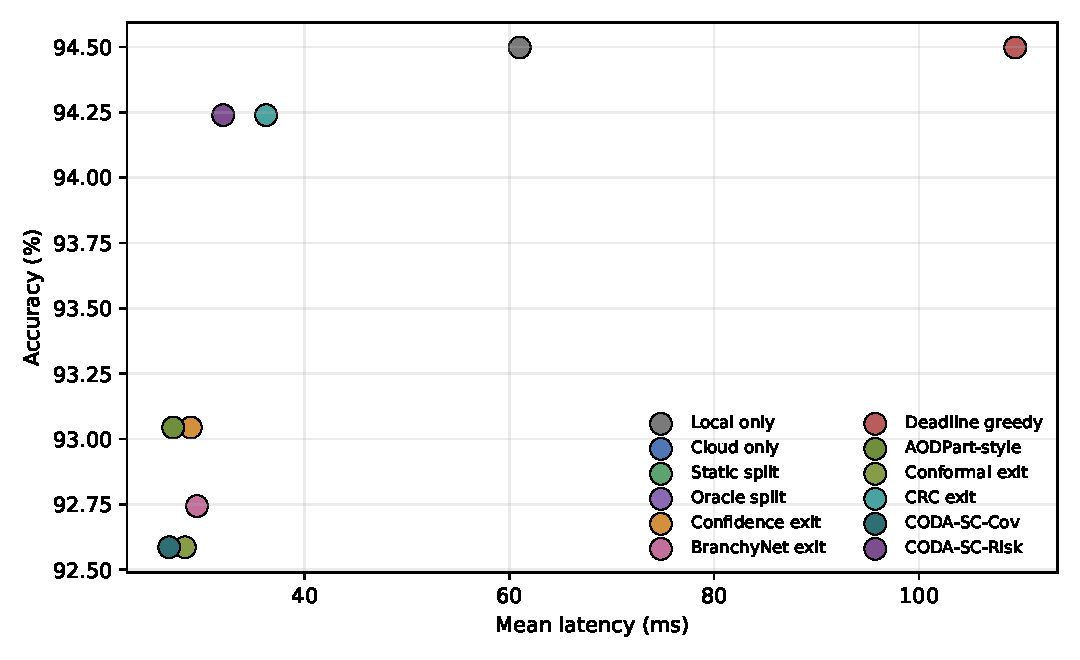
\includegraphics[width=0.48\linewidth]{results/latency_accuracy.pdf}
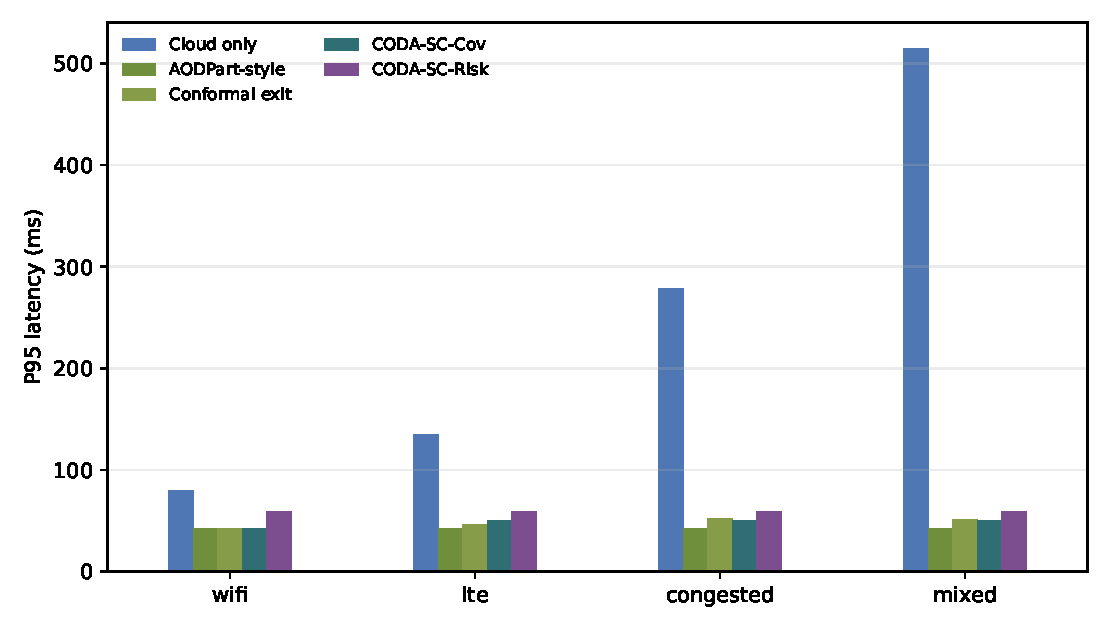
\includegraphics[width=0.48\linewidth]{results/p95_by_profile.pdf}\\
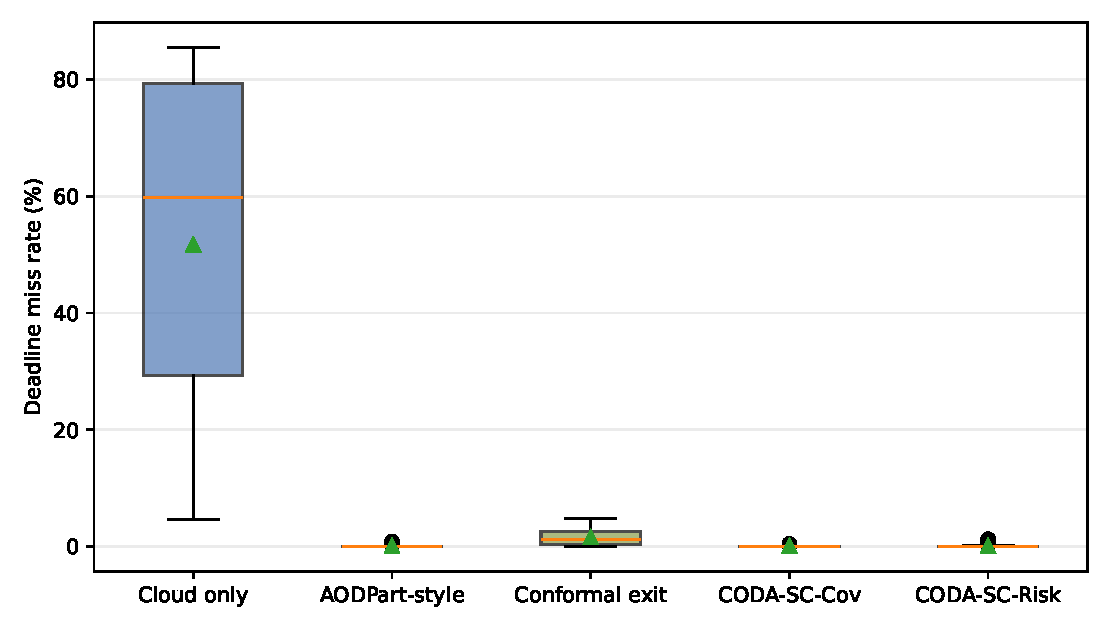
\includegraphics[width=0.48\linewidth]{results/miss_box.pdf}
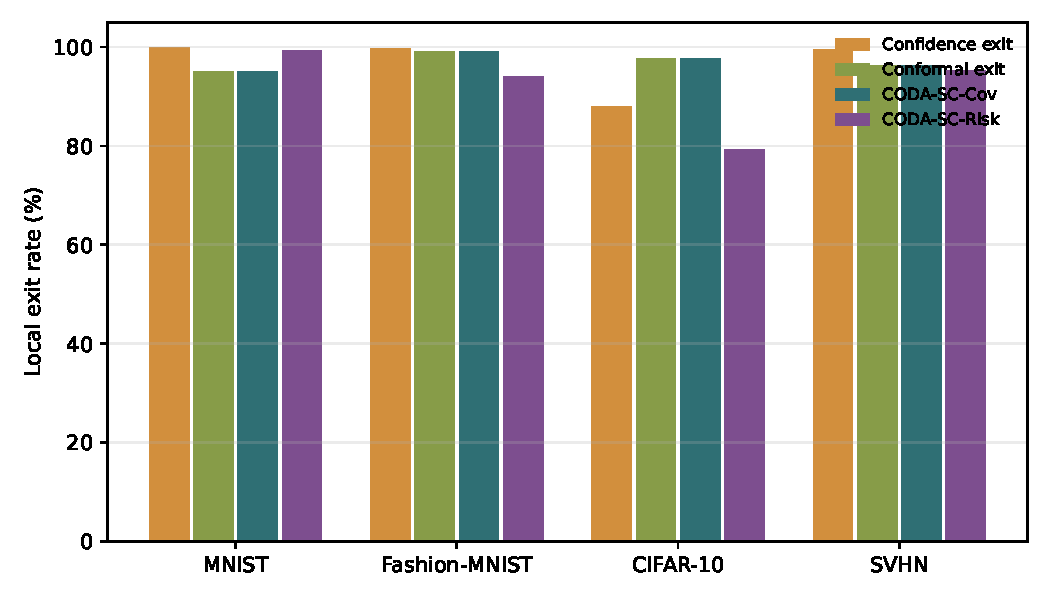
\includegraphics[width=0.48\linewidth]{results/exit_by_dataset.pdf}
\caption{Top left: latency-accuracy trade-off averaged across profiles. Top
right: profile-specific P95 latency for network-dependent methods. Bottom left:
distribution of deadline-miss rates across dataset$\times$seed$\times$profile,
showing that CODA-SC removes the congested-profile tail that cloud-only suffers.
Bottom right: local exit rate by workload, which stays high (95--99\%) across the
difficulty range so that most requests avoid the network entirely.}
\label{fig:results}
\end{figure}

\subsection{Confidence versus conformal exits}

At matched operating points, confidence-threshold and conformal exits are
competitive on accuracy and empirical selective error, and neither is uniformly
superior across workloads. The distinguishing property of conformal exits is not lower
empirical error but a finite-sample, distribution-free coverage result
(Theorem~\ref{thm:cov}) and an explicit selective-error control
(Proposition~\ref{prop:crc}) that a confidence threshold does not provide. The
conformal-risk-control variant makes this explicit: it targets a selective-error
level directly and trades exit rate for reliability accordingly. Thus the
empirical claim is not that conformal exits are consistently faster or more
accurate than tuned confidence exits, but that they expose a reliability contract
that can be composed with deadline-aware control.

\subsection{Sensitivity}
\label{sec:sens}

Supplementary Table S3 sweeps the conformal level $\alpha$ and the edge
throughput $\Phi_{\mathrm{e}}$. Smaller $\alpha$ lowers selective error but
reduces the local exit rate, shifting more traffic to the controller; a weaker
edge device raises local compute cost and therefore the value of offloading when
the network is healthy. The qualitative conclusions are stable across the sweep,
but the absolute deadline-miss rate is sensitive to edge throughput. This is
expected: CODA-SC deliberately uses local execution as a deadline-safe fallback,
so its benefit depends on the device being fast enough to complete the fallback
before the deadline.

\subsection{Discussion}

The results establish a hierarchy of evidence. The main benchmark supports the
calibrated selective-control mechanism: local conformal exits provide most of
the latency and upload reduction, and the coupled controller suppresses deadline
misses on the small residual stream by switching between offload and local
fallback. It does not, by itself, demonstrate broad advantages for intermediate
split selection. On these small-image workloads, early activation tensors can be
larger than the raw input, so the controller often chooses between raw offloading
and local computation rather than among many intermediate split points. This
explains why cloud-only, static split, oracle-split, and deadline-greedy policies
have similar aggregate latency in Table~\ref{tab:main}: without compression or
larger inputs, intermediate split points do not create a meaningful payload
advantage.

The learned-bottleneck study in Table~\ref{tab:bottleneck} addresses a narrower
question: whether the action space can express useful split decisions when
intermediate representations are compressed by a trained codec. It strengthens
the split-selection evidence relative to payload scaling alone because the
accuracy of a split action is now produced by the decoded suffix. It also shows
the cost of such compression: the split-only policies obtain lower upload and
lower latency than raw cloud offload in the high-resolution regime, but at a
substantial accuracy loss with this small codec. The present evidence should
therefore be read in three levels: strong support for calibrated early exits and
residual fallback/offload control; diagnostic support for learned compressed
split actions and their accuracy-latency trade-off in the same simulated setting;
and no claim of deployment-level hardware validation.

\section{Limitations and Future Work}

The benchmark is reproducible on standard CPU/GPU infrastructure, but it is not a
hardware deployment study. Activation payloads and FLOPs are exact for the
trained models; edge and cloud throughputs are documented modelling assumptions,
and the sensitivity study shows that these assumptions materially affect
deadline misses. Network latency is trace-simulated from bandwidth, RTT,
queueing, and loss processes rather than measured on a live wide-area edge-cloud
deployment, so operational effects such as diurnal load, routing changes, server
contention, and correlated failures are not captured. The learned bottlenecks
are lightweight 1$\times$1 codecs trained on the same 32$\times$32 vision
workloads; they validate the compressed-action interface but are not a phone or
edge-server measurement, and they do not replace a high-resolution deployment
study with hardware codec timing. The theoretical statements are marginal and
depend on exchangeability of calibration and test examples; they do not by
themselves protect against distribution shift, label shift, or adaptive
adversarial inputs. Finally, the experiments are limited to feed-forward vision
classification.
Autoregressive foundation models introduce token-level scheduling, KV-cache
placement, and speculative decoding decisions that require a different action
space.

\section{Conclusion}

CODA-SC formulates split inference as a joint selective-prediction and online
control problem. Conformal exits determine when an intermediate prediction is
eligible for local output; a primal-dual controller determines how to handle the
remaining requests under deadline, upload, and energy costs. On four multi-exit
CNN vision workloads with simulated Internet-like traces, the method reduces
mean latency and deadline misses relative to cloud-only and split-only policies,
while exposing a reliability interface that confidence-only early exits lack.
The gains are not free: frequent early exits reduce accuracy relative to full
inference, the local fallback relies on sufficient edge throughput, and the
calibration statements require exchangeability. The learned-bottleneck study
shows how compressed intermediate actions can be evaluated with decoded-suffix
predictions, but direct high-resolution and hardware experiments are still
needed before claiming deployment-level split-selection gains. Future work
should replace the device model with direct phone/edge measurements, evaluate
adaptive conformal calibration under distribution shift, add stronger learned
activation compression for high-resolution workloads, and extend the action
space to autoregressive foundation-model inference.

\section*{Reproducibility Statement}

All code needed for the experiments is included in this workspace. The main
command is:
\begin{verbatim}
python3 scripts/run_experiments.py --seeds 7,13,29,42,101 --repeats 6 \
  --enable-learned-bottlenecks --bottleneck-channels 8 \
  --bottleneck-epochs 8 --output results
\end{verbatim}
It trains the multi-exit CNNs (if not cached), trains the frozen-backbone split
bottlenecks, measures the systems profiles, evaluates all policies over the
network traces, and regenerates the CSV summaries, calibration diagnostics,
LaTeX tables, figures, and graphical abstract included in this manuscript.
Dataset splits, network traces, and initialization are controlled by fixed seeds.

\section*{Data Availability Statement}

The code, cached model outputs, generated CSV summaries, LaTeX tables, figures,
and diagnostics are available at
\url{https://github.com/pz1004/coda-sc-public}. The experimental artifacts can
be regenerated with the command in the reproducibility statement above. Public
dataset sources are downloaded by the scripts where permitted by their original
licenses; no proprietary data are used.

\section*{CRediT Author Statement}

To be completed before submission with the final author names and roles
(Conceptualization, Methodology, Software, Validation, Formal analysis,
Investigation, Data curation, Writing -- original draft, Writing -- review and
editing, Visualization, Supervision, Project administration, and Funding
acquisition as applicable).

\section*{Declaration of Competing Interest}

The authors declare that they have no known competing financial interests or
personal relationships that could have appeared to influence the work reported
in this paper.

\section*{Funding}

This research received no external funding.

\section*{Declaration of Generative AI and AI-assisted Technologies in the Writing Process}

During the preparation of this work the authors used OpenAI Codex for editorial
revision planning, consistency checking, and manuscript editing support. After
using this tool, the authors reviewed and edited the content as needed and take
full responsibility for the content of the publication.

\bibliographystyle{plainnat}
\bibliography{references}

\end{document}
